\section{Component Densities}

\begin{figure}[h!]
\begin{center}
	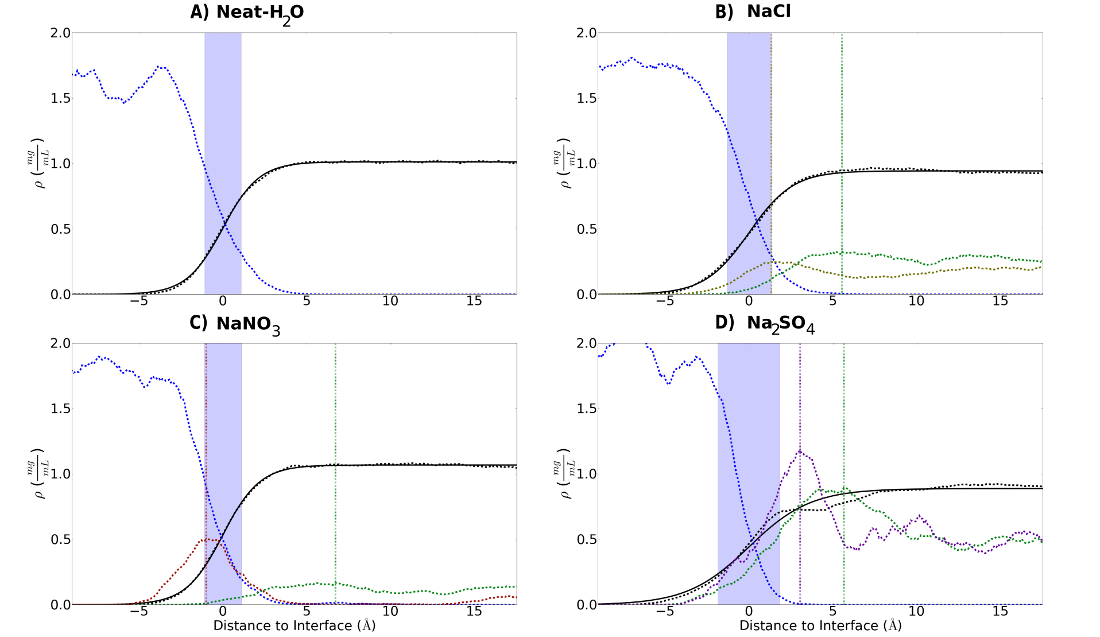
\includegraphics{images/densities.png}
	\caption{Aqueous salt solution (1.2 M) and \ctc surface density profiles. (A) Reference \ctcwat, (B) NaCl, (C) \sodnit, and (D) \sodsul aqueous solution densities are plotted with the water-oxygen density (dashed black) and the corresponding fitted lineshape (solid black). The \ctc (dashed blue), Na$^+$ cation (dashed green, scaled 10x) and respective anion (scaled 5x) densities are also shown for each system. The maxima of the ionic components are marked with dashed vertical lines of the same colors.}
	\label{fig:density-plots}
\end{center}
\end{figure}

The component density profiles of each system were calculated to study the effects of added salts on water's density profile, and to find any deviations in the behavior of water from the \ctcwat system. The water density profile of each system was fitted to a hyperbolic tangent function (Eq. \ref{tanh_fit}). The resulting plots are shown in Figure \ref{fig:density-plots}. The profiles were centered about the GDS locations, $z_0$, at 0.0\angs, and all lineshapes are plotted as distances to the GDS. Each interfacial width, $d$, is designated as a highlighted blue region of width $d$ centered about $z_0$.  The widths of the interfacial regions for the neat-\ctcwat (A), NaCl (B), NaNO$_3$ (C), and Na$_2$SO$_4$ (D) systems are 2.16, 2.62, 2.20, 3.69\angs, respectively. In each of the salt solutions, the anion density profile shows higher density near the interface, appearing as a peak in the density profile. These anion enhancements all occur closer to the interface than the corresponding counter-cation density enhancement. 

%*
It is important to note from our density calculations that ions that increase the interfacial width at the \ctcwat interface correspond to ions that result in an enhancement of the SFG signal from interfacial water. As discussed later, our SFG calculations show excellent agreement with experimental results that also show this enhancement for such ions. Also, we find those ions that are best known to enhance the strength of hydrogen-bonding (i.e. \sul) produce wider interfaces with greater water penetration into the \ctc phase.

Various parameters of interest such as the interfacial thicknesses, ionic enhancement locations (taken to be the location of the maxima in the ion profiles), and relative distances between the peaks of the ion profiles are collected in Table \ref{table:double-layer}.

\begin{table}[htdp]
	\begin{center}
	\begin{tabular}{|c||c|c|c|c|}
		\hline
		System & $d$ & Anion & Cation & Anion-Cation Distance \\ \hline
		Neat-H$_2$O & 2.16 & - & - & - \\ 
		NaCl & 2.62 & 1.33 & 5.53 & 4.20 \\
		NaNO$_3$ & 2.20 & -0.99 & 6.71 & 7.70 \\
		Na$_2$SO$_4$ & 3.69 & 3.04 & 5.64 & 2.60 \\
		\hline
	\end{tabular}
	\end{center}
	\caption{Aqueous salt system density parameters. Interfacial widths, $d$, and the locations of the maxima of the density profiles for each ionic component are listed for the simulated salt systems. The relative distances between the anion and cation density peak locations are listed to show how the different anions affect the relative location of their cationic counter-ions.}
	\label{table:double-layer}
\end{table}

The oscillations in the surface density profiles of water and the adjoining organic \ctc liquid phase have been noted previously and attributed to thermal capillary waves on a larger length-scale than the simulated system size.\cite{Chang1996} The same work also made note that the interfacial thickness is size-dependent on the interfacial surface area. Increasing the surface area dimensions should therefor cause a proportional increase in the interfacial width. As a consequence, care must be taken when making quantitative comparisons between widths and locations found in differing simulation studies. However, relative width ordering between similarly-sized systems should remain, as shown in two separate works on the \ctcwat surface.\cite{Chang1996,Hore2008}

%*1
% ********comparison to air-water**********
% Use this paragraph to talk about the differences with the AIR-water systems, and back it up with stuff found from calculations
The majority of liquid surface studies examining ion behavior over the past decade have been conducted on \airwat interfaces. A recent review elucidates the convergence of data and conclusions regarding \airwat systems, paying special attention to relevant computational efforts.\cite{Jungwirth2006a} Ion behavior at liquid-liquid interfaces, however, is clearly different than these \airwat computational studies. The large polarizable and monovalent anions (\cl, Br$^-$, I$^-$) undergo concentration enhancement above bulk levels at the \airwat interface more than at the organic interface.\cite{Wick2006c,Wick2007a} 

%*2
A break in the isotropic environment around the ions causes them to be less solvated and come in greater contact with the \ctc phase. The ions are thus pushed further into the aqueous bulk and more hydrated than at an air-interface. However, the surface activities and ion density enhancements of the more polarizable anions (i.e. I$^-$, Br$^-$) remain greater than that of a smaller and less polarizable one (i.e. Cl$^-$) at both interfaces. 

%3
In comparing the three salt solutions studied here, any differences in these systems are the result of the anion because the same cation was used in each system. \nacl is the simplest of the three salts with a monatomic and monovalent anion. The peak of the anion density profile is within the aqueous phase (i.e. it is found on the aqueous-side of the interfacial width). The location of the cation density peak is, as mentioned above, deeper into the aqueous phase than the anion by over 4\angs. This layering of ions within the aqueous phase is attributed to the break in the isotropy of the field of the bulk region upon introduction of the organic phase. From our studies it is clear that polarizable monovalent anions move towards the interface and effectively screen the induced field from the organic phase. The counter-ions then are drawn towards the negative charge built up by the anions to create the second ion density peak deeper in the aqueous phase. The overall shape of the water profile in the \nacl system is relatively unaffected (compared to the neat-\ctcwat) by the presence of the ions. The width of the interface is slightly increased above that of the reference system.


%4a,b
The \sodnit system introduces the monovalent, polyatomic nitrate anion. The behavior of molecular anions such as \nit at \airwat has been explored recently with computer simulation,\cite{Thomas2007,Miller2009} spectroscopy,\cite{Soule2007,Xu2009,Otten2007} and depth-resolved X-ray photoemission spectroscopy.\cite{Brown2009} Studies tend to agree that the \airwat surface affinity of the \nit anion is no greater than the water bulk (i.e. for large simulated systems), but conclusions differ on the extent of density depletion or enhancement. The large planar geometry of the \nit anion and its low charge appear to repel it from the \airwat surface where it encounters a reduced solvent cage, and seeks a more hydrated solvation state. In comparison the \nit does alter the \ctcwat interface with its density greatly enhanced within the surface region above bulk levels. Also, a wide ionic double-layer is established with its counter-ion left deeper in the aqueous bulk. In our simulation we find a strong surface density enhancement of the nitrate anion. The nitrate density peak is located the furthest out from the aqueous phase of the three salt systems, as expected by its higher polarizability and low charge. The location of the sodium cation peak in this system is a significant distance further into the bulk water relative to the anion than in either of the \nacl or \sodsul systems. The increase in ion-pair distance is likely the result of strong screening of the interfacial field by the surface-active anion, and the solvating waters around it. The interfacial width of the \sodnit system is the narrowest relative to the other salts in this study. 

%4c
It is likely that slight reorientation of the surface waters near \ctc enhance the solvation of the \nit in the plane of the interface and establish a much more hydrated region for the anion to adsorb. Water reorientation is more fully described later in this work. The subsurface waters then continue to screen the charge of the surface-active \nit, and decrease the coulombic force pulling the cation closer to the surface. 

%5
The widest interface is that of the \sodsul solution, indicating that the \sul anions act to increase the number of interfacial water molecules on both sides of the GDS, consistent with the highly solvated nature of \sul and its larger size. \sul density enhancement (the peak of the anion density profile) is furthest into the aqueous bulk of the three anions simulated. The calculations suggest that the divalent and highly polarizable nature of the \sul anion attracts its counter-ion closest, leading to the narrowest sub-surface ionic double-layer. This attraction is likely coulombic. Although the greatest anionic concentration enhancement is further into the bulk water region, seemingly outside the region designated by the interfacial width, the water interfacial width is still greatly enhanced. This is in agreement with the experimental \sodsul SFG studies where sulfate ion leads to an enhanced SFG signal throughout the bonded OH stretch region, consistent with a larger interfacial width.\cite{McFearin2009}

Unlike the monovalent ions, the divalent \sul anion has a very large first solvation shell and prefers a location deeper into the aqueous phase at the \airwat interface,\cite{Salvador2003} and is perhaps repelled from the interfacial region.\cite{Gopalakrishnan2005} This more highly-solvated anionic behavior coincides with the \ctcwat system seen here. Although the presence of the \ctc changes the interfacial environment from that of the \airwat interface, the field established by the deep aqueous-side location of the \sul anion density enhancement acts to affect the interface from a greater distance. 

Ionic double-layers at both \airwat and \ctcwat surfaces have been documented in many of the studies already referenced. The distance between the anion and cation subsurface enhancements at the \ctcwat interface are shown in Table \ref{table:double-layer}. An SFG study by Schultz et al. using similar sodium salts noted the double-layer at the \airwat interface and attributed it to a ``displacement'' mechanism binding ions to interfacial waters, and forming contact-ion pairs. This was based on the lower-frequency OH vibrational mode found at 3150\cm, and the lack of signal change with added salts. Since then Xu et al studied this phenomena with an SFG experiment finding no ion-pairing in solution of various nitrates with divalent cations at the \airwat interface.\cite{Xu2009} The same study probed the vibrational modes of the \nit anion, rather than water's OH modes finding two anionic surface species. They concluded that solvation from an abundance of water at the interface weakens coulombic forces between ions, leading to greater cation-anion separation. The surface nitrate is dehydrated, and the water provides adequate shielding of the ionic coulombic interactions. We find ion double-layering at the \ctcwat interface with no contact-ion pair formation for each of the salts. Likely, this is due to the stronger reorientation of water in the presence of the organic phase, and the subsequent field-screening by sub-surface waters between the ionic layers.

